\documentclass{article}

% if you need to pass options to natbib, use, e.g.:
%     \PassOptionsToPackage{numbers, compress}{natbib}

\usepackage[utf8]{inputenc} % allow utf-8 input
\usepackage[T1]{fontenc}    % use 8-bit T1 fonts
\usepackage[colorlinks,allcolors=blue]{hyperref}       % hyperlinks
\usepackage{url}            % simple URL typesetting
\usepackage{booktabs}       % professional-quality tables
\usepackage{amsfonts}       % blackboard math symbols
\usepackage{nicefrac}       % compact symbols for 1/2, etc.
\usepackage{microtype}      % microtypography

% Additional packages
\usepackage{amsmath}
\DeclareMathOperator{\Normal}{\mathrm{Normal}}

\usepackage{algorithm}
\usepackage[noend]{algpseudocode}

% for fancy Mike style table
\usepackage[table]{xcolor} 
\usepackage{multirow}

\usepackage{tikz}
\usepackage{float}
\usepackage{wrapfig}

\newtheorem{theorem}{Theorem}

\title{sbc}

% The \author macro works with any number of authors. There are two commands
% used to separate the names and addresses of multiple authors: \And and \AND.
%
% Using \And between authors leaves it to LaTeX to determine where to break the
% lines. Using \AND forces a line break at that point. So, if LaTeX puts 3 of 4
% authors names on the first line, and the last on the second line, try using
% \AND instead of \And before the third author name.

\author{%
}

\begin{document}

\maketitle

\begin{abstract}

\end{abstract}


\section{SBC on adjoint-differentiated Laplace}

\citep{margossian2020hamiltonian} has proposed an algorithm that combines HMC with Laplace approximation. This could achieve both greater speed and less tuning efforts, and therefore accuracy, compared to the standard model especially for latent gaussian models with poisson and bernoulli likelihood. SBC could diagnose the validity of this algorithm and further provide a feedback for improvement, if any. In the context of validating the approximation algorithm, we are assuming the standard model, our approximation target, as the true data generating process. Then approximation model is applied to fit the M simulated set of y values.  


 \subsection{Disease map and Poisson likelihood with log link}
 
\citep{Vanhatalo+Pietilainen+Vehtari:2010} models the mortality count across Finland. Data is aggregated in n = 911 counties. For speed issues, 20 randomly selected counties are used. As prior parameters should be set by the modeler, different sets in terms of mean and standard deviation $\alpha$ and $\rho$ are expermented. As can be seen from the Figure-\ref{fig:dmSBC}, all are within the bound of credible interval, which signifies the 0.005 quantile to the 0.995 quantile of the $\operatorname{Binomial}\left(N,(L+1)^{-1}\right)$ distribution. Bins is the number of bins whose values is 20, following the recommendation of \citep{Talts:2018}. It is expected that, on average, the counts in only one bin a hundred will deviate outside this shaded interval. The different shapes of SBC histogram and average fitting time between them could be explained through difference in simulated y values. For example, the simulated set y1 in Figure-\ref{fig:ysimExtreme}, took more than 10 times longer to fit compared to other simulated y value sets.   
 
  \begin{figure}[!htb]
  \centering
    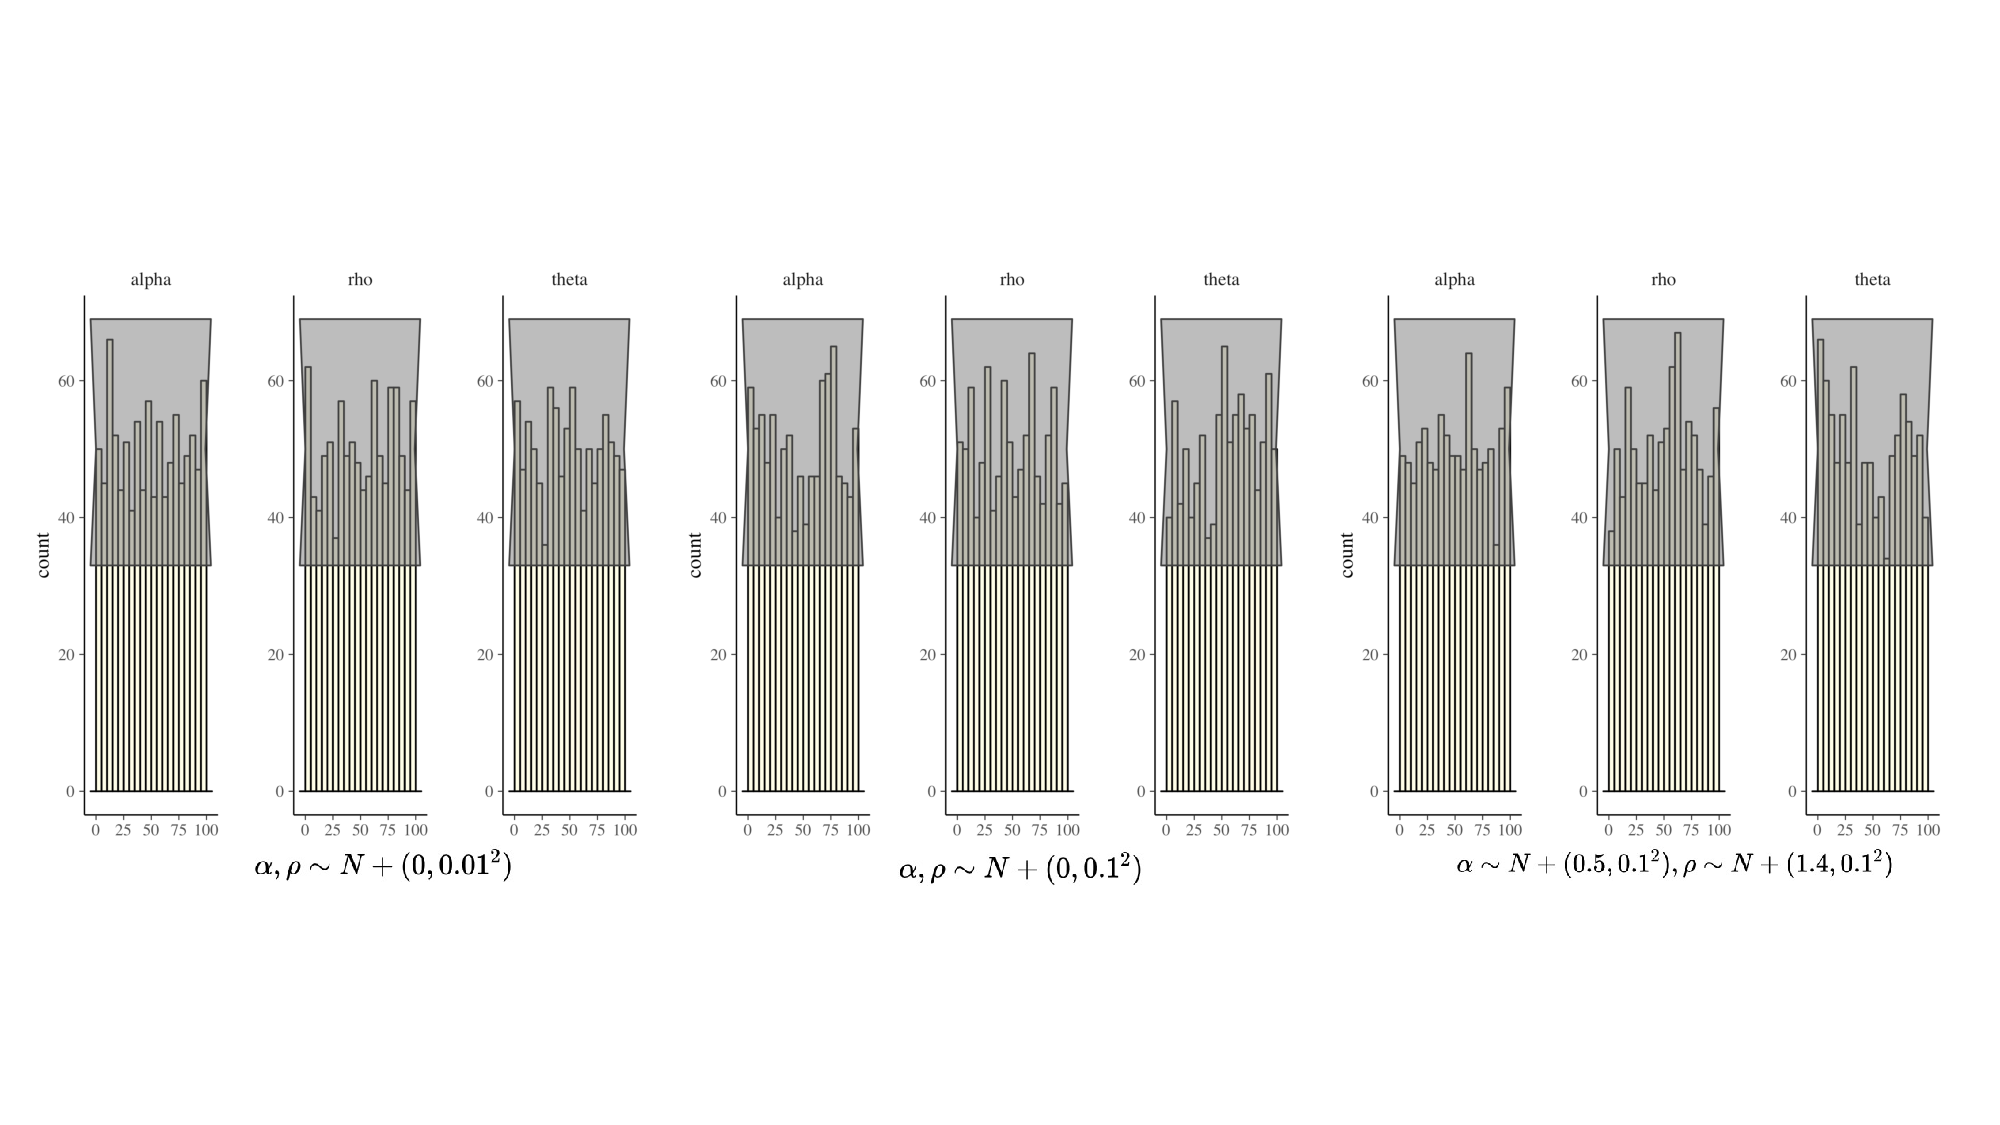
\includegraphics[width=\textwidth]{figures/diseasemap_sbc.pdf}
    \caption{SBC histogram for disease map data with different prior parameter input}
    \label{fig:dmSBC}
  \end{figure}
  
  \begin{figure}[!htb]
  \centering
    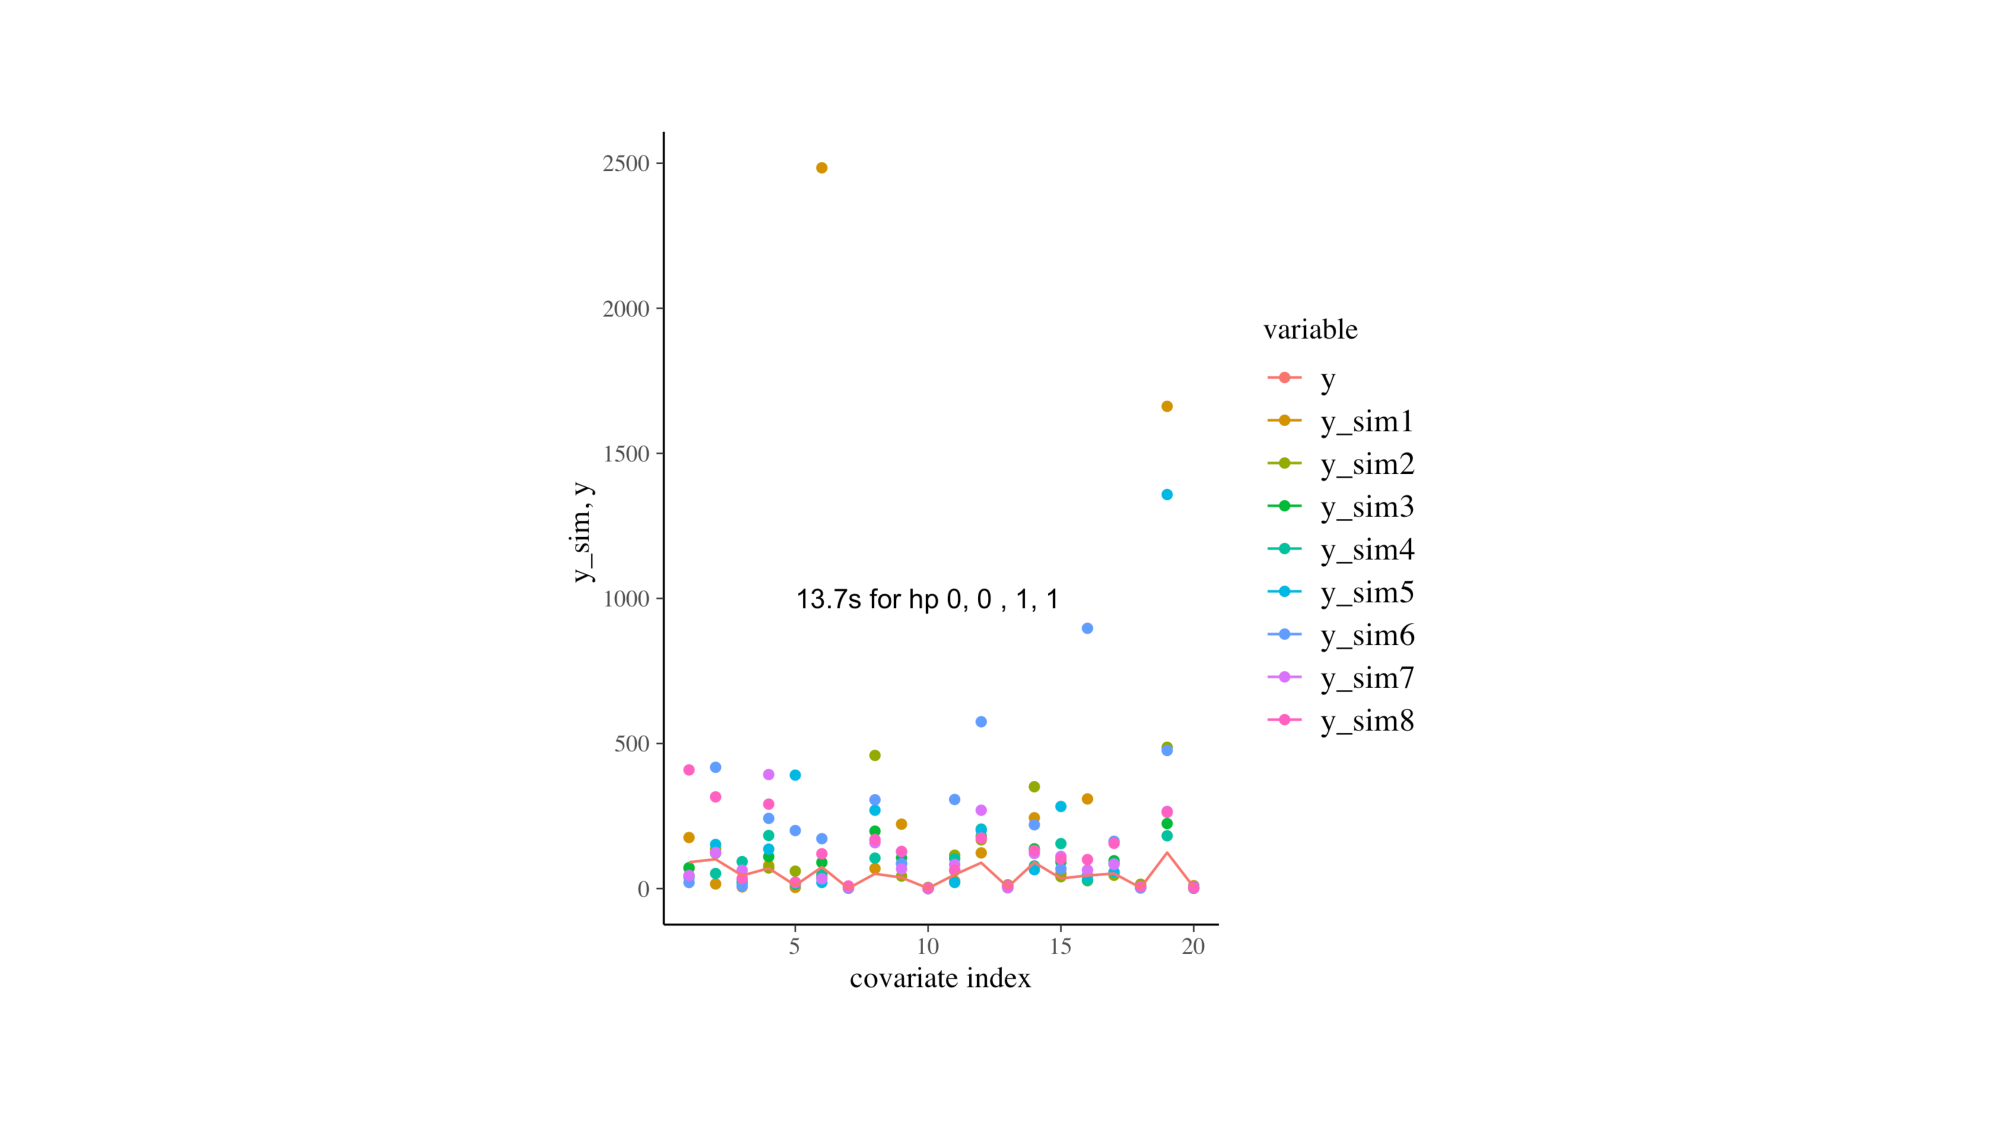
\includegraphics[width=\textwidth]{figures/y_sim_extreme.pdf}
    \caption{Simulated y values for different prior parameter input}
    \label{fig:ysimExtreme}
  \end{figure}
  
 Figure \ref{fig:ysimPriorParam} shows the average fitting time and simulated y values for each prior parameters for $\alpha$ and $\rho$. Empirically learned values, 0.5 and 1.4( $\alpha$ and $\rho$ each) are plugged in for the mean parameter to be compared with mean 0. Note that as half normal priors are used, mean would not be exactly the same, especially for mean 0. Lower scale values tend to result in a faster fit with more realistic simulated y values. How much variance in simulated y values is appropriate in terms of testing the algorithm is a subject that needs further discussion. On the other hand, different location values do not have a clear tendency with average fitting time, though y values simulated from smaller mean value tend to be closer to real y values. However, though this realistic values have a clear relationship with average fitting time, this do not necessarily lead to better uniformity which could be seen from \ref{fig:pvalPriorParam}.
 

  
  \begin{figure}[!htb]
  \centering
    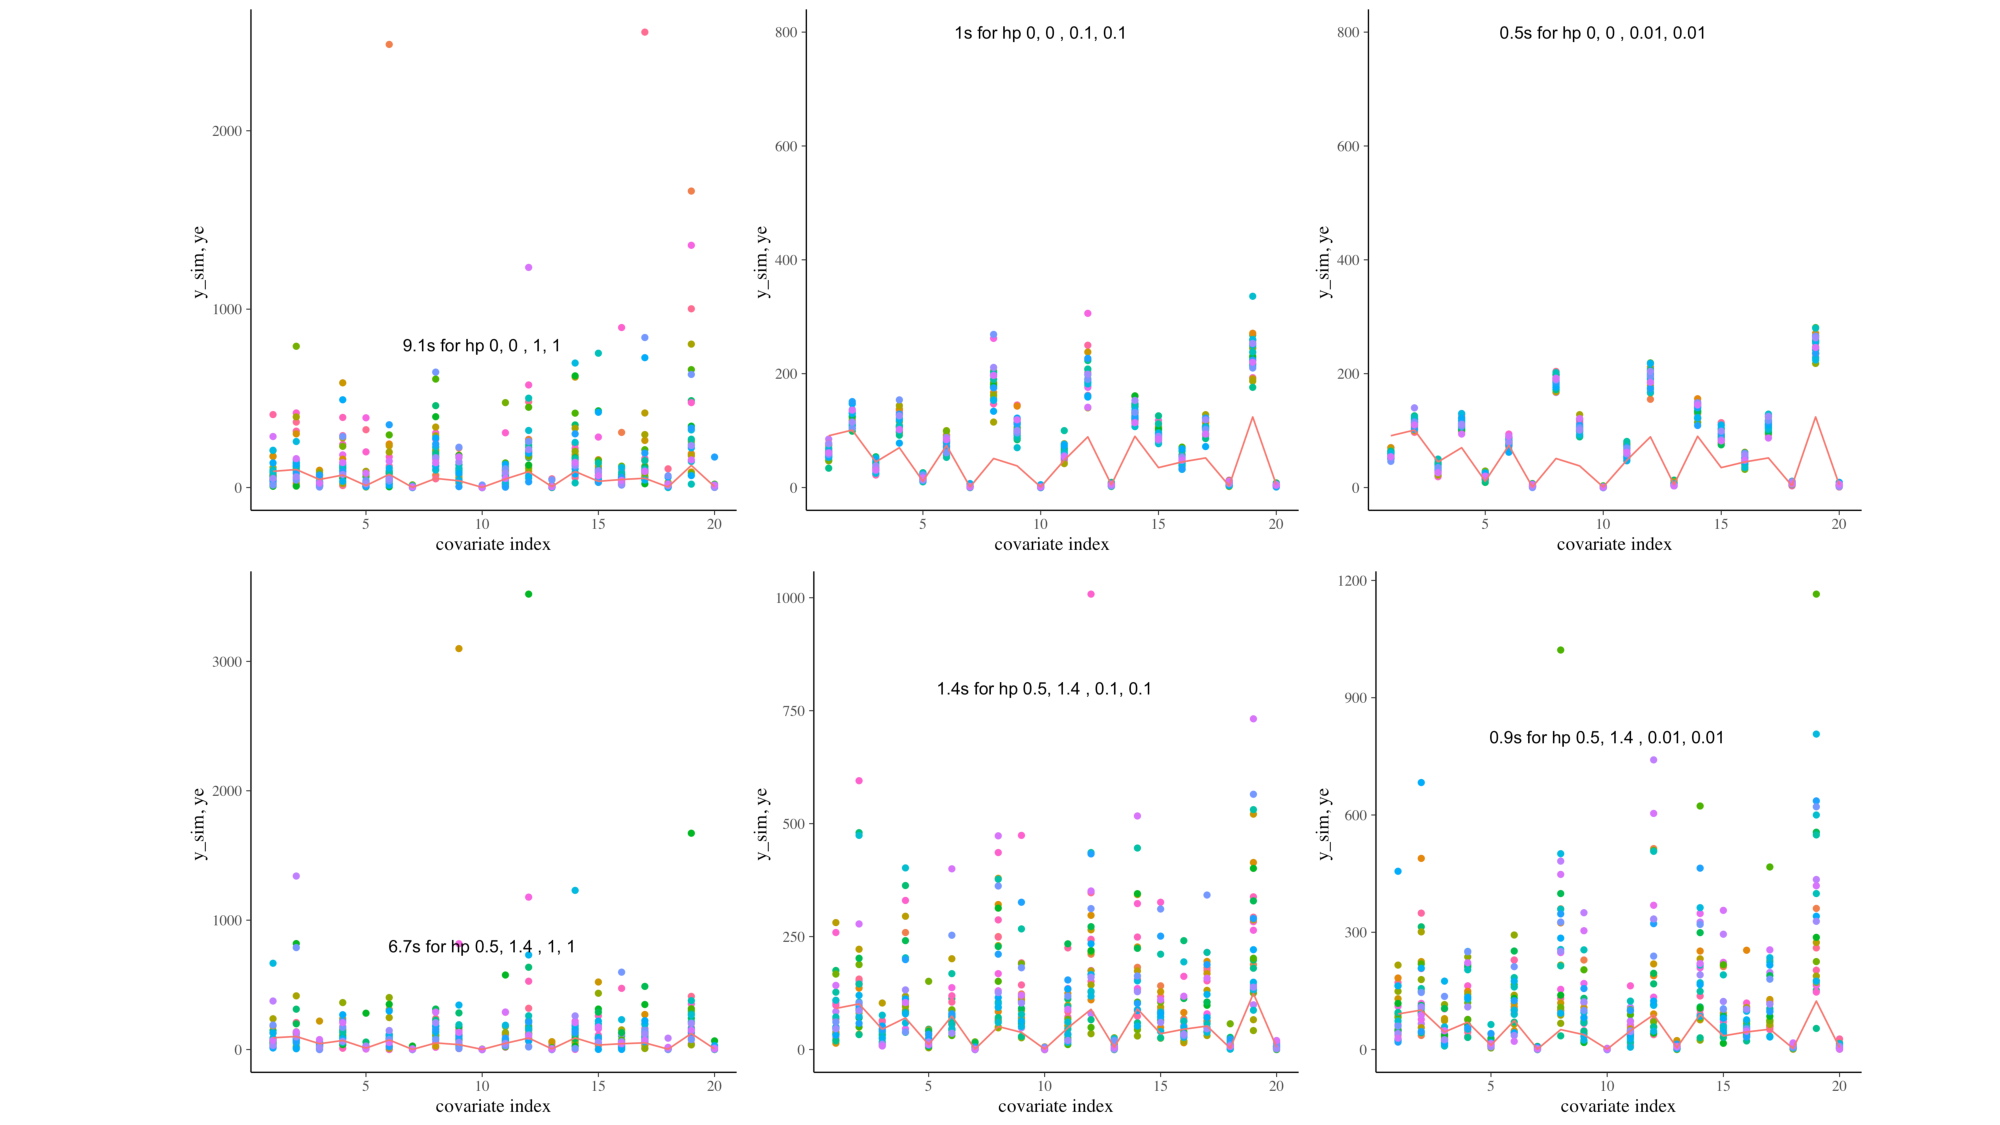
\includegraphics[width=\textwidth]{writeup/figures/y_sim_prior_param.pdf}
    \caption{Simulated y for different prior parameter input with real y}
    \label{fig:ysimPriorParam}
  \end{figure}
  
  
   \begin{figure}[!htb]
    \centering
    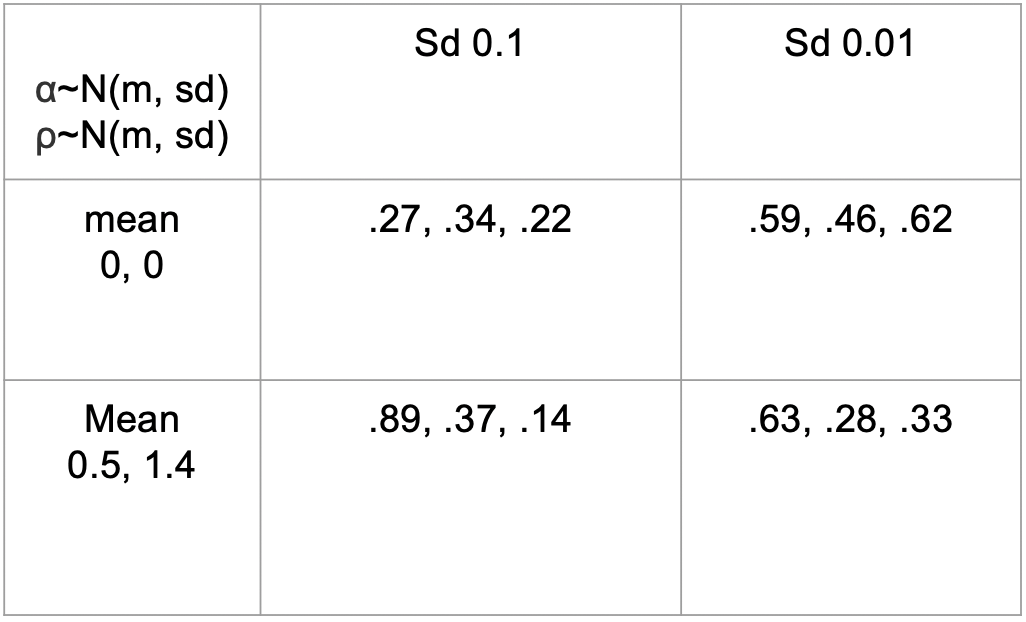
\includegraphics[width=\textwidth]{writeup/figures/diseasemap_pval.png}
    \caption{SBC uniformity pvalues for different prior parameter input}
    \label{fig:pvalPriorParam}
  \end{figure}
  
  
Half normal distribution was used for Figure \ref{fig:ysimPriorParam}, but it is worth noting that using half-t or inverse gamma with the same first and second moment led to different SBC results. Different symmetry and tail behaviors are expected to have caused these differences in y values (Figure \ref{fig:ysimPriorShape}) and therefore SBC results  (Figure \ref{fig:SBCPriorShape}. Also, different pvalues and averaged fitting times are reported. Fitting time: .90s, .85s, 1.9s / Pvalues: (.67, .49, .82),(0.90, 0.58, 0.81), (.13, 0, .74) for $\alpha$,$\rho$, $\theta1$ [normal, t, and inverse gamma ( mean 0.42, 1.1 / variance 3.6e-05)]. $\rho$ parameter for inverse gamma prior is interesting (Figure \ref{fig:SBCPriorShape}).

  \begin{figure}[!htb]
  \centering
    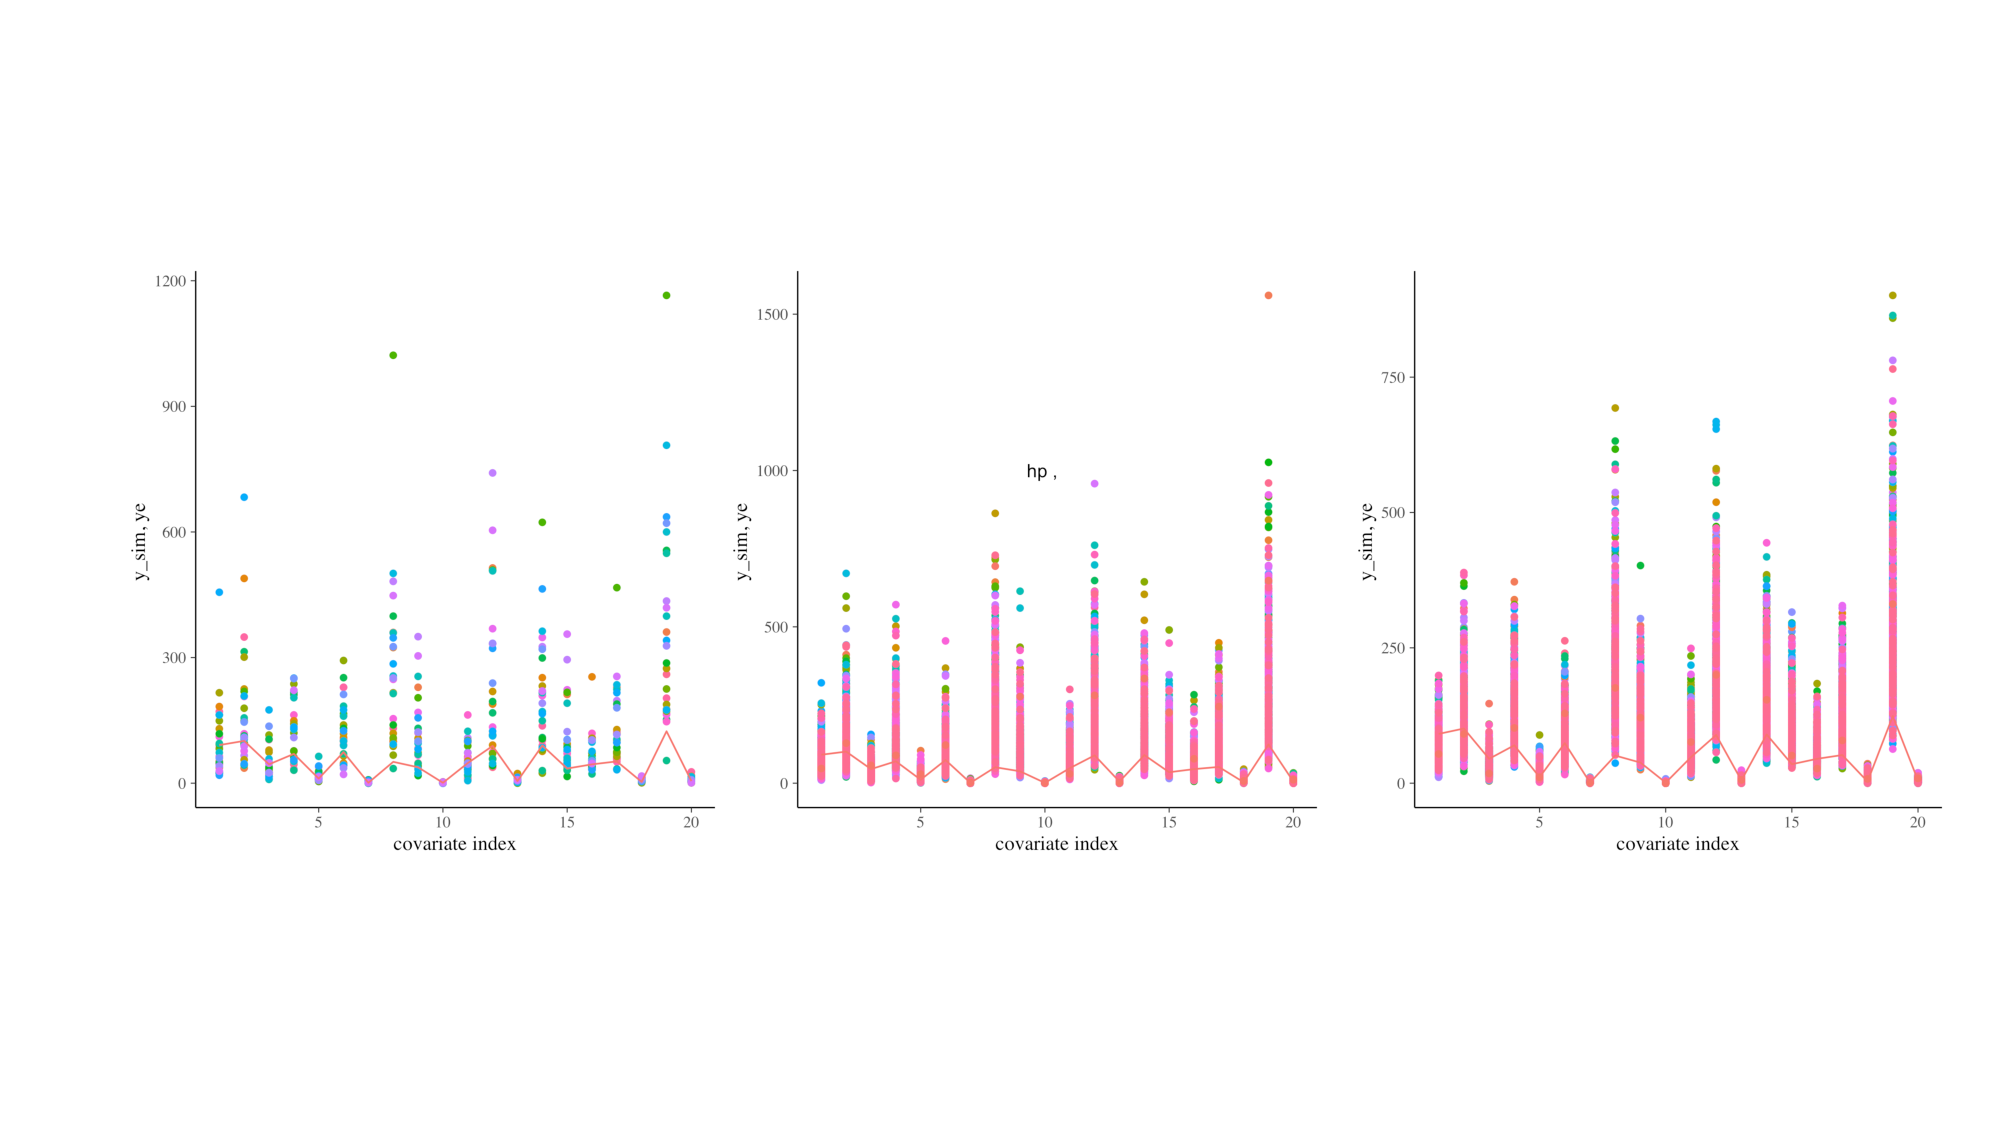
\includegraphics[width=\textwidth]{writeup/figures/dm_y_sim_priorshape.pdf}
    \caption{simulated y values for different prior shape}
    \label{fig:ysimPriorShape}
  \end{figure}
  
  \begin{figure}[!htb]
  \centering
    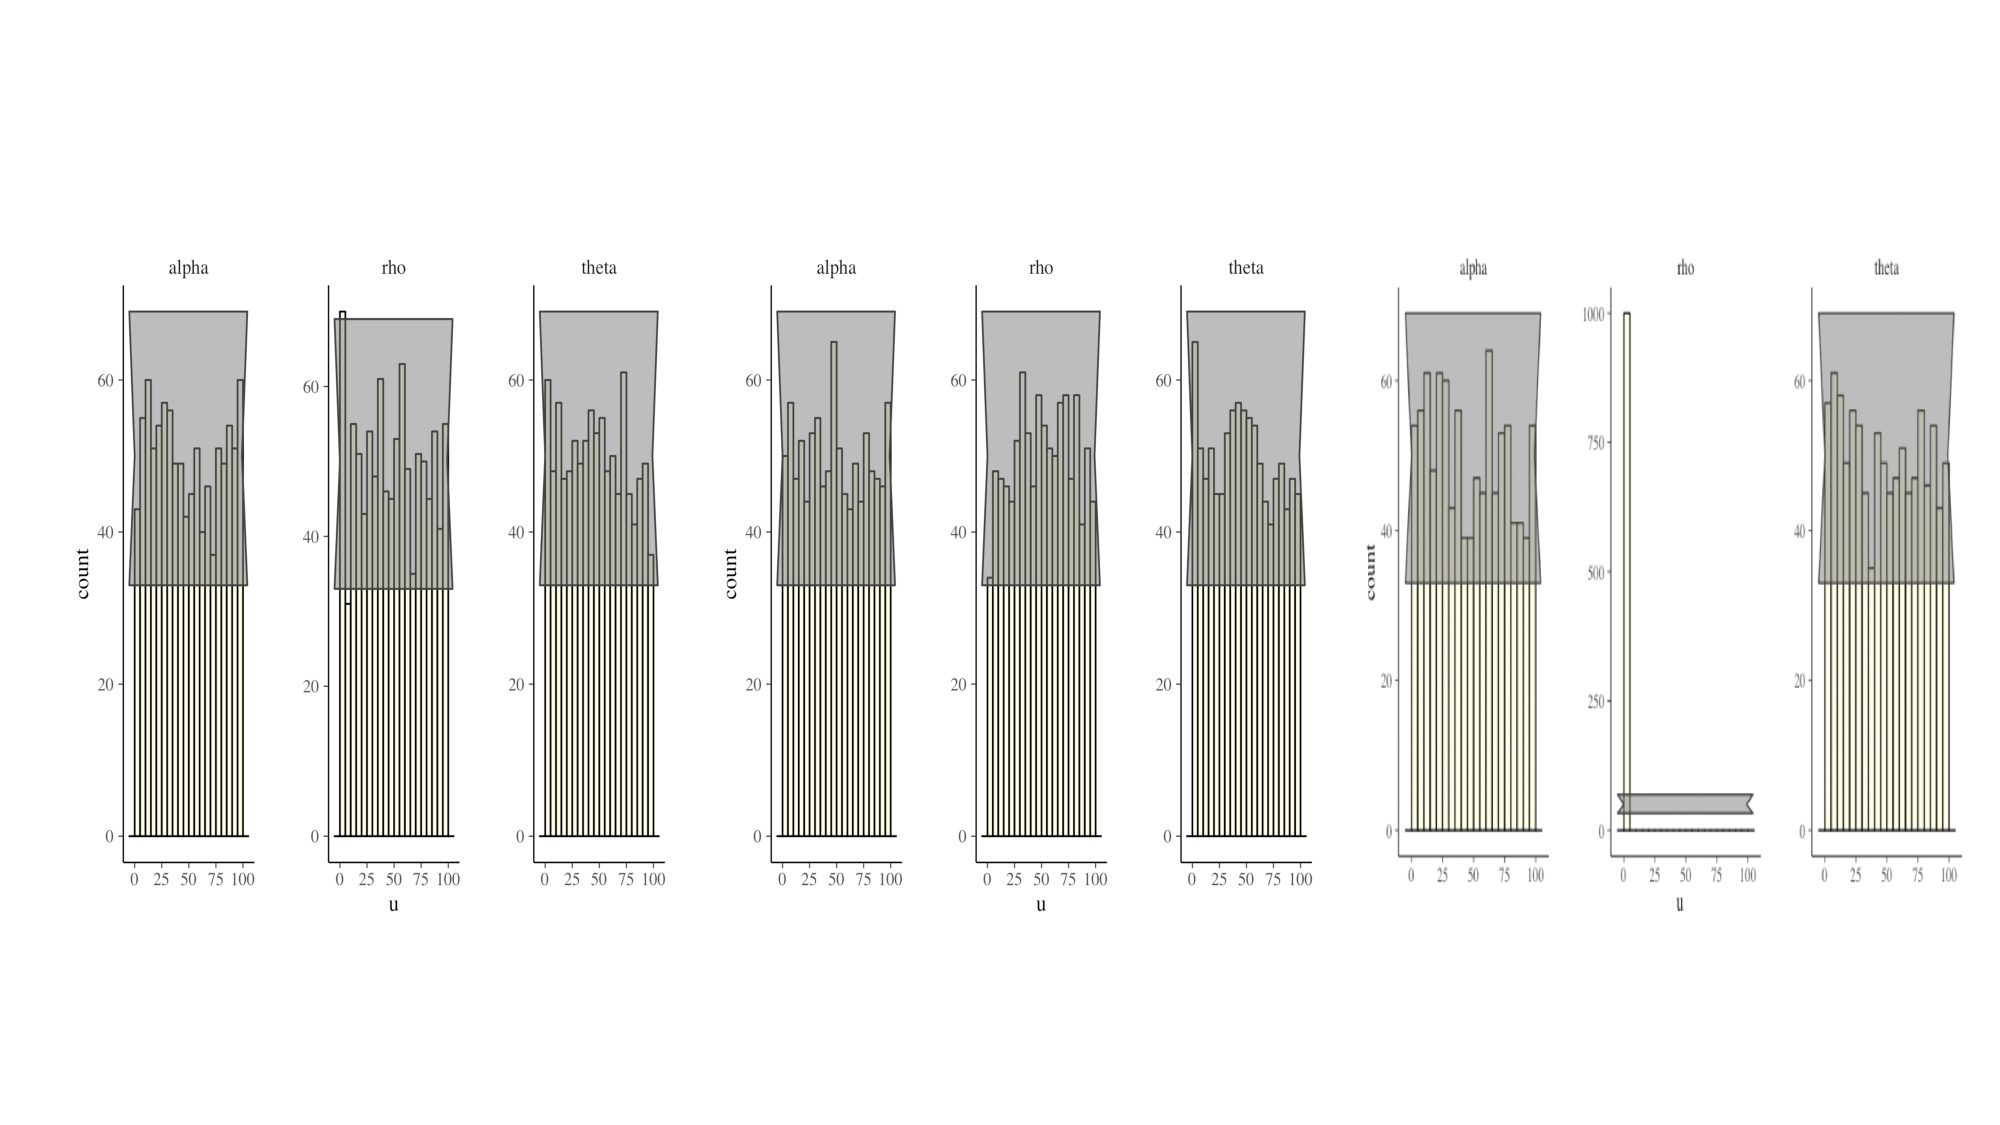
\includegraphics[width=\textwidth]{writeup/figures/diseasemap_sbc_priorshape.pdf}
    \caption{SBC histogram for different prior shape}
    \label{fig:SBCPriorShape}
  \end{figure}


 \subsection{Cancer factors and Bernoulli likelihood with logit link}
  For Bernoulli likelihood, general linear regression model with a regularized horseshoe prior is used. Figure \ref{fig:hhSBC}, shows SBC histogram of selected five parameters. lambda1 and 86 each represents coefficient for minor and major cancer factor. p[1] is probability of the first patient getting a cancer. 
  
  For parameters whose SBC histograms flagged some problems, simulated and fitted values were compared. Note that underscored are prior samples. As can be seen from Figure~\ref{fig:hhLambda}, both major and minor factors showed the tendency to overestimate the values. For the probability of certain patients getting a cancer, the approximation algorithm showed tendency to balance out the probability between two extremes, 0 and 1 (Figure~\ref{fig:hhProb1}). It is expected that for patients with higher risk of cancer, the SBC histogram bias would look the same except for the bias direction; most ranks would be concentrated on the right. This is not surprising as Laplace model is known to avoid extreme values of the probability.
  
    \begin{figure}[!htb]
  \centering
    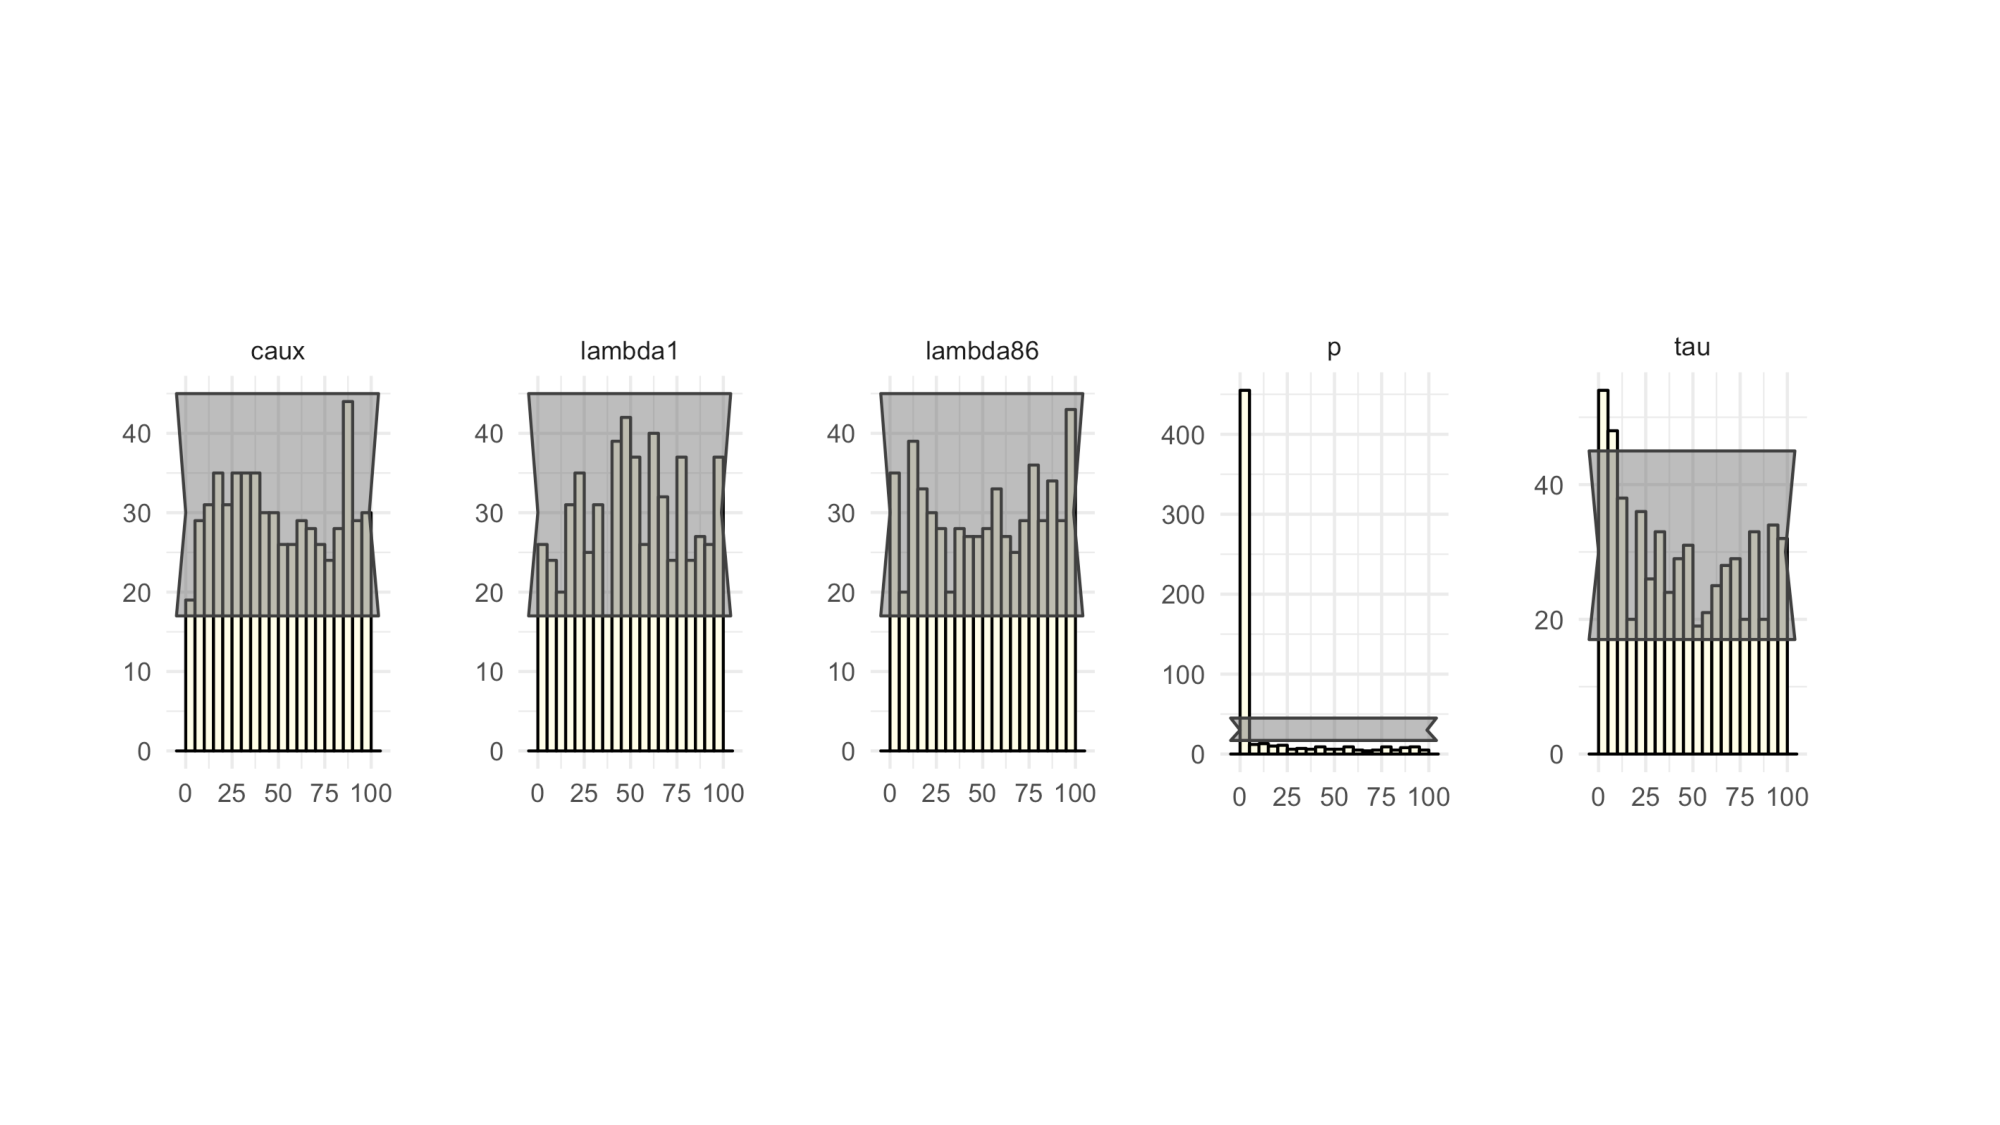
\includegraphics[width=\textwidth]{writeup/figures/horseshoe_sbc.pdf}
    \caption{SBC histogram for prostate cancer data}
    \label{fig:hhSBC}
  \end{figure}
  
  \begin{figure}[!htb]
  \centering
    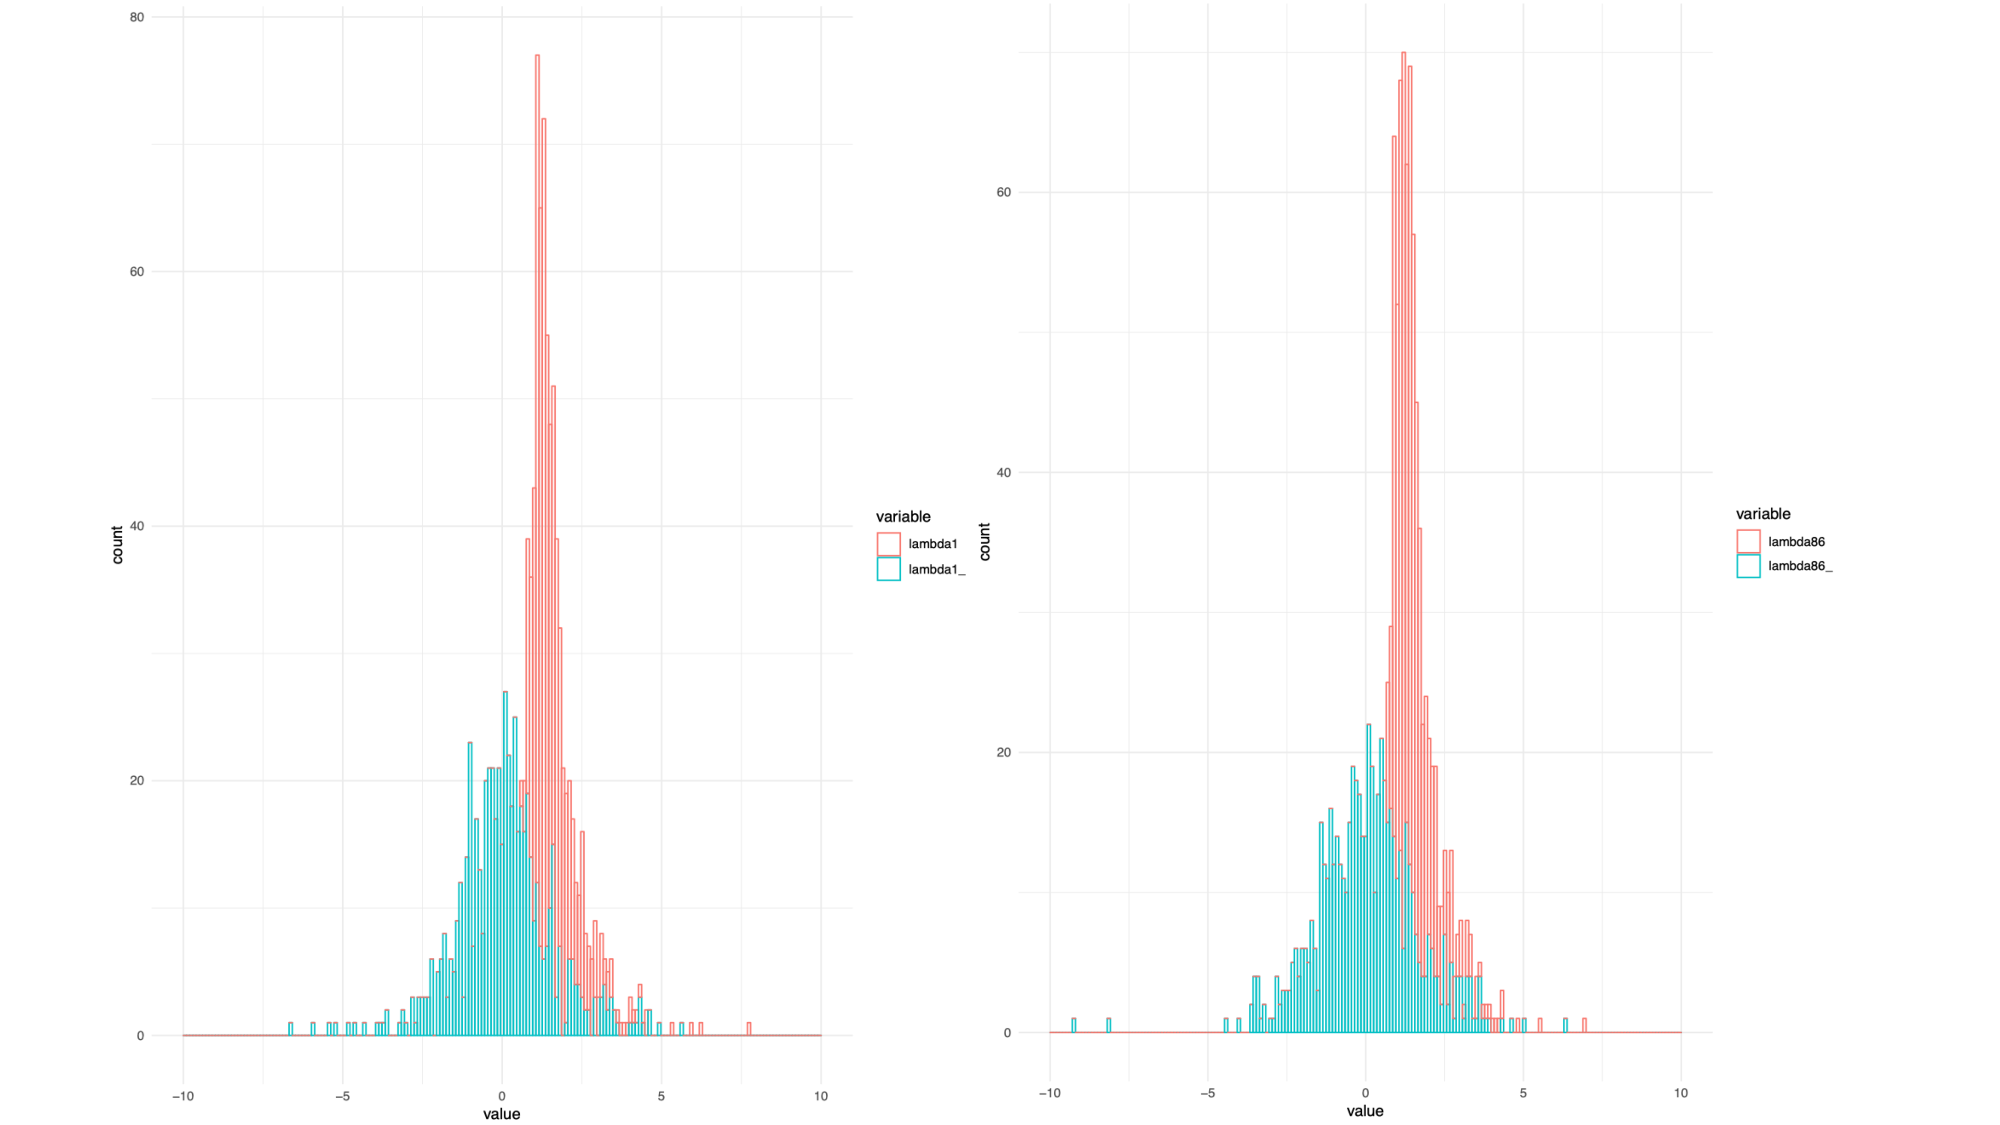
\includegraphics[width=\textwidth]{writeup/figures/horseshoe_lambda1_86.pdf}
    \caption{Compare simulated lambda with lambda posterior samples of each fit(mean) of a factor}
    \label{fig:hhLambda}
  \end{figure}
  
  \begin{figure}[!htb]
  \centering
    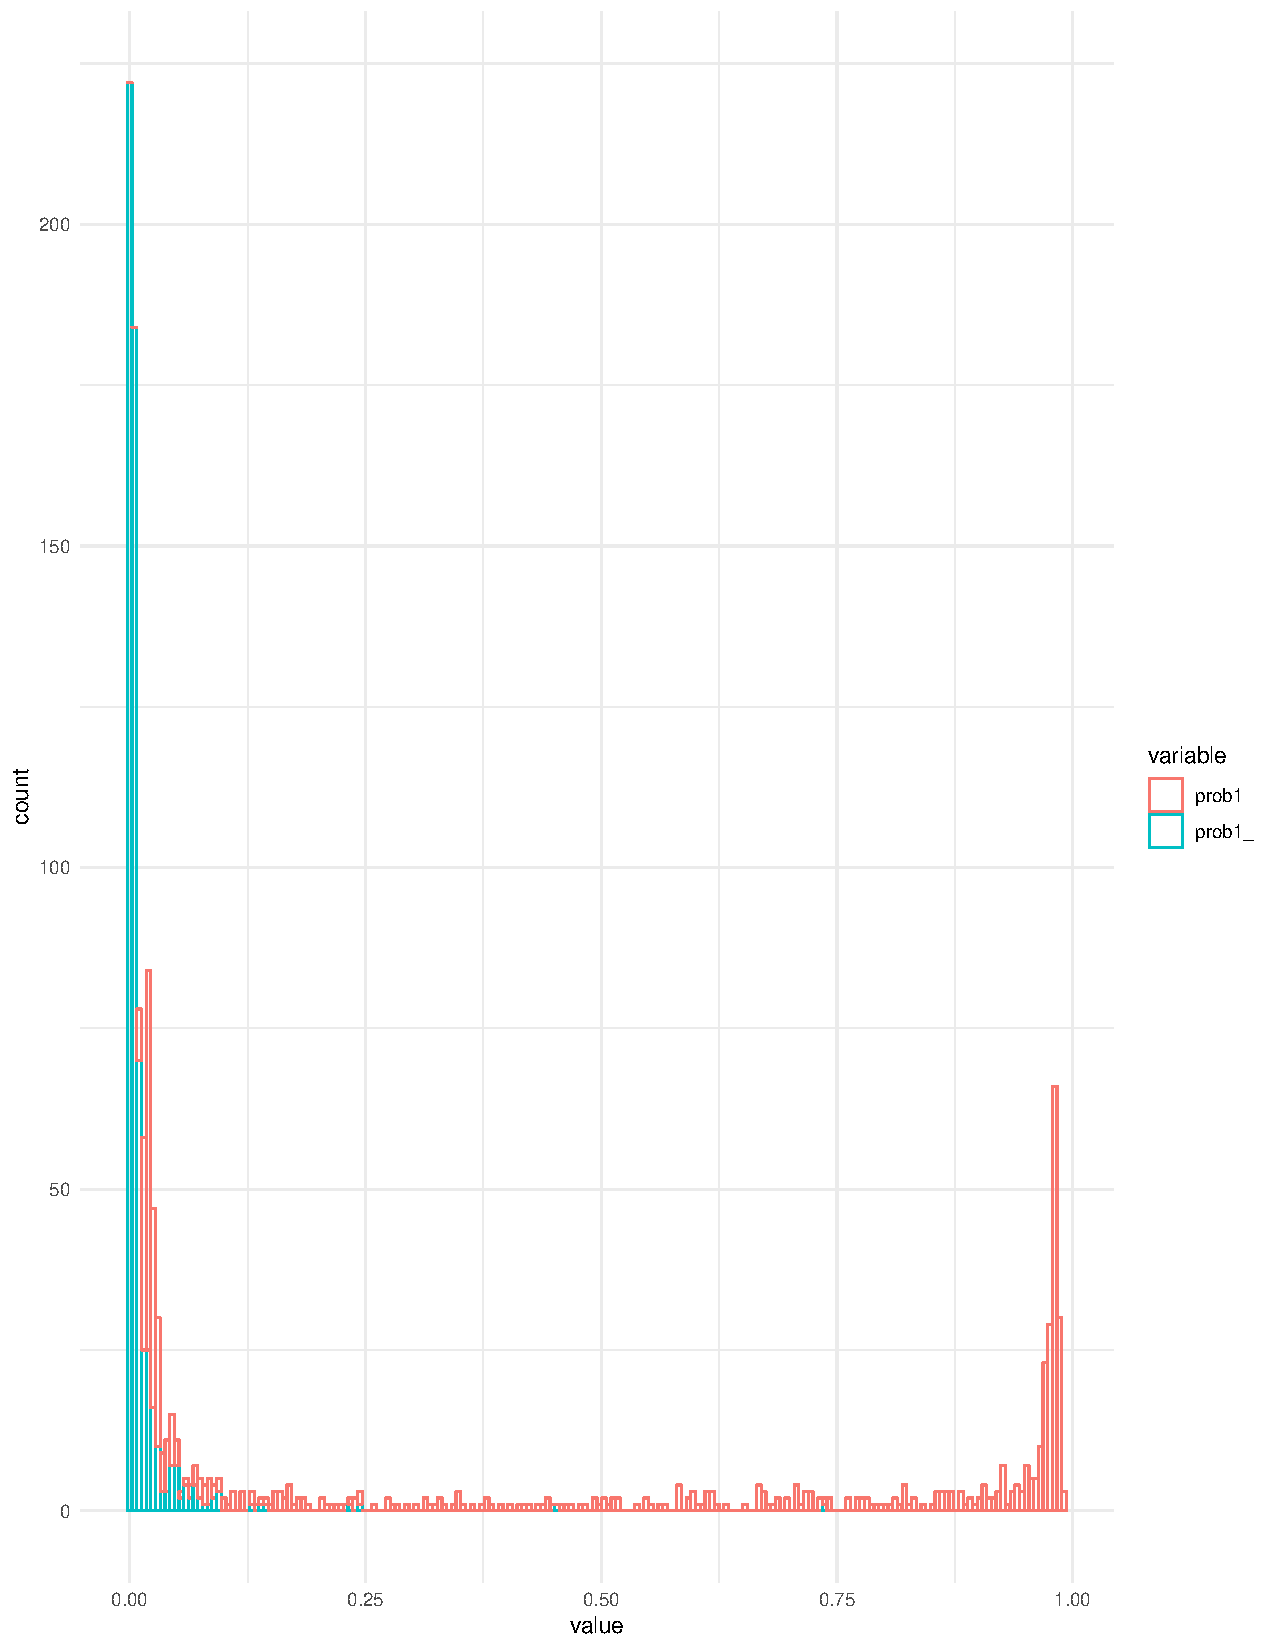
\includegraphics[width=\textwidth]{writeup/figures/horseshoe_prob1.pdf}
    \caption{Compare simulated cancer probability with its posterior samples of each fit(mean)}
    \label{fig:hhProb1}
  \end{figure}
  
  
  
  \bibliography{ref_sbc.bib}
 % \bibliographystyle{abbrvnat}
  \bibliographystyle{imsart-nameyear}
  
 
\end{document}

